\begin{center} 
\emph{``To raise new questions, new possibilities, to regard old problems from a new angle, requires creative imagination and marks real advance in science.'' --  Albert Einstein}
\end{center}

\section{Orthogonal Projections}\label{sec:orthoproj}
\begin{Thm}[Parseval's Identity]\label{5} Let  $S= \{\bb v_1, \ldots, \bb v_p\} \subseteq F^n$ be an orthogonal subset. If $\bb y$ is a linear combination of the vectors in $S$, that is, 
\[\bb y = c_1\bb v_1 + c_2\bb v_2 + \ldots + c_p\bb v_p,\] then \[c_i = \dfrac{\bb v_i \cdot \bb y}{\bb v_i \cdot \bb v_i},\quad\text{called the \textbf{Fourier coefficients}.}\]
\end{Thm}
\begin{proof}
Taking the dot product, we get 
\[\bb v_i\cdot \bb y = \bb v_i \cdot (c_1\bb v_1 + c_2\bb v_2 + \ldots + c_p\bb v_p) = c_i(\bb v_i \cdot \bb v_i).\] Since $\bb v_i\cdot \bb v_i\neq 0$, dividing both sides by $\bb v_i\cdot \bb v_i$ gives the formula.
\end{proof}\vs

\begin{Exam} Let $S = \left\{\bb v_1 = (1,2,3), \bb v_2 = (1,1,-1), \bb v_3 = (-5,4,-1)\right\}$, which was shown in \examref{exam:4.2orthobasis} to be an orthogonal subset of $\R^3$. By \thmref{thm:orthoindependent}, we see that $S$ is, in fact, an orthogonal basis for $\R^3$. Let $\bb y = (-4,8,10)$. Since $\bb y \in \R^3$, $\bb y$ is a linear combination of the vectors of $S$. By \thmref{5}, we have 
\begin{eqnarray*}
\bb y &=& \left(\dfrac{\bb v_1 \cdot \bb y}{\bb v_1 \cdot \bb v_1}\right)\bb v_1 + \left(\dfrac{\bb v_2 \cdot \bb y}{\bb v_2 \cdot \bb v_2}\right)\bb v_2 + \left(\dfrac{\bb v_3 \cdot \bb y}{\bb v_3 \cdot \bb v_3}\right)\bb v_3 = \dfrac{42}{14}\bb v_1 + \dfrac{-6}{3}\bb v_2 + \dfrac{42}{42}\bb v_3 = 3\bb v_1 - 2\bb v_2 + \bb v_3 \\
&=& 3\vr{1\\2\\3} - 2\vr{1\\1\\-1} + \vr{-5\\4\\-1} = \vr{-4\\8\\10}, \text{ that is, } [\bb y]_S = \vr{3\\-2\\1}.
\end{eqnarray*}
\end{Exam}


%Every vector $\bb v \in \R^2$ has two components: the \emph{horizontal component} $v_1$ and the \emph{vertical component} $v_2$, that is, $\bb v = \vr{v_1\\v_2}$.  These components uniquely determine $\bb v$. Let $\bb{v_x} = \vr{v_1\\0}$ and $\bb{v_y}  = \vr{0\\v_2}$. These are the unique vectors in the direction of the $x$-  \vspace{-0.1 in}
%\begin{multicols}{2}\noindent
% and $y$-axes, respectively, such that $\bb v_x + \bb v_y = \bb v$. The vectors $\bb{v_x}$ and $\bb{v_y}$ are the shadows that $\bb v$ casts on the $x$- and $y$-axes, respectively. They are also orthogonal. It turns out that this orthogonal decomposition can be done in general.%\columnbreak

%\mbox{}\vspace{-0.25 in}
%\begin{center}
%\begin{tikzpicture}
%\draw[dashed, ultra thick, gray] (0,2) -- (3,2);
%\draw[dashed, ultra thick, gray] (3,0) -- (3,2);
%\draw[->, ultra thick] (0,0) -- (3,0) node[midway, below right] {$\bb v_x$};
%\draw[->, ultra thick] (0,0) -- (0,2) node[midway, above left] {$\bb v_y$};
%\draw[->, ultra thick, red] (0,0) -- (3,2) node[midway, above] {$\bb v$};
%\end{tikzpicture}
%\end{center}
%\end{multicols}

\begin{Def} Let $\bb y\in F^n$ and $W\le F^n$. Let $\{\bb u_1,\ \bb u_2,\ \ldots, \bb u_r\}$ be an orthogonal basis for $W$. Then the \textbf{orthogonal projection} of $\bb y$ onto $W$ is 
\[\widehat{\bb y} = \proj_W \bb y = \sum_{i=1}^r\dfrac{\bb u_i \cdot \bb y}{\bb u_i\cdot \bb u_i}\bb u_i = \dfrac{\bb u_1 \cdot \bb y}{\bb u_1\cdot \bb u_1}\bb u_1 + \dfrac{\bb u_2 \cdot \bb y}{\bb u_2\cdot \bb u_2}\bb u_2+ \ldots + \dfrac{\bb u_r \cdot \bb y}{\bb u_r\cdot \bb u_r}\bb u_r.\] When the subspace $W$ is clear from context, $\proj_W(\bb y)$ is often abbreviated as $\widehat{\bb y}$.\\

Let $\bb y,\ \bb u \in F^n$ and $\bb u \neq \bb 0$.  Then the \textbf{orthogonal projection} of $\bb y$ onto $\bb u$ is $\proj_{\bb u} \bb y = \proj_W \bb y$, where $W = \Span(\bb u)$. 
\end{Def}\vs

\begin{multicols}{2}
Intuitively, the orthogonal projection of $\bb y$ onto $\bb u$ is the shadow the arrow $\bb y$ casts on the line spanned along $\bb u$.\\

\mbox{}\vspace{-0.25 in}
\begin{center}
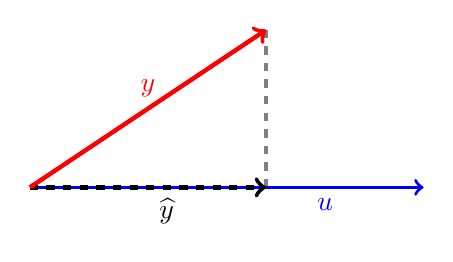
\begin{tikzpicture}
\draw[dashed, ultra thick, gray] (3,0) -- (3,2);
\draw[->, very thick, blue] (0,0) -- (5,0) node[near end, below] {$\bb u$};
\draw[->, ultra thick, dashed] (0,0) -- (3,0) node[midway, below right] {$\widehat{\bb y}$};
\draw[->, ultra thick, red] (0,0) -- (3,2) node[midway, above] {$\bb y$};
\end{tikzpicture}
\end{center}
\end{multicols}

\begin{Exam} Let $\bb y = \vr{1\\7\\3}$ and $\bb u = \vr{2\\1\\1}$. Then 

\[\widehat{\bb y} = \proj_{\bb u}(\bb y) = \dfrac{\bb u\cdot \bb y}{\bb u \cdot \bb u}\bb u = \dfrac{12}{6} \vr{2\\1\\1} =  \vr{4\\2\\2}.\] Note that \[\bb y - \widehat{\bb y} = \vr{1\\7\\3} - \vr{4\\2\\2} = \vr{-3\\5\\1},\qquad \bb y = \widehat{\bb y} + (\bb y - \widehat{\bb y}) = \vr{4\\2\\2} + \vr{-3\\5\\1},\] and that \[\widehat{\bb y} \cdot (\bb y - \widehat{\bb y}) = \vr{4\\2\\2}\cdot \vr{-3\\5\\1} = -12+10+2=0.\] Therefore, $\bb y - \widehat{\bb y}$ and $\widehat{\bb y}$ are orthogonal, that is, $\bb y - \widehat{\bb y}\in W^\perp$.
\end{Exam}\vs

%\begin{Thm} Let $\bb y, \bb a \in \R^n$ and $\bb a\neq \bb 0$. Then 
%\[\proj_{\bb a} \bb y \cdot (\bb y - \proj_{\bb a} \bb y) = 0.\]
%\end{Thm}
%\begin{proof}
%\begin{eqnarray*}
%\proj_{\bb a} \bb y \cdot (\bb y - \proj_{\bb a} \bb y) &=& \proj_{\bb a} \bb y \cdot \bb y - \proj_{\bb a} \bb y \cdot \proj_{\bb a} \bb y\\
% &=& \dfrac{\bb y \cdot \bb u}{\bb u \cdot \bb u}(\bb u \cdot \bb y) -  \left(\dfrac{\bb y \cdot \bb u}{\bb u \cdot \bb u}\bb u\right)\cdot \left(\dfrac{\bb y \cdot \bb u}{\bb u \cdot \bb u}\bb u\right)\\
%&=& \dfrac{(\bb y \cdot \bb u)^2}{\bb u \cdot \bb u} - \dfrac{(\bb y \cdot \bb u)^2}{(\bb u \cdot \bb u)^2}(\bb u \cdot \bb u) = 0.
%\end{eqnarray*}
%\end{proof}

%If $\bb u\neq \bb 0$, then $\{\bb u\}$ is automatically an orthogonal basis for $W=\Span\{\bb u\}$. In this case, $=\proj_{\bb u}(\bb y) = \proj_W(\bb y)$. Intuitively, the orthogonal projection of $\bb y$ onto $\bb u$ is the shadow the arrow $\bb y$ casts on the line spanned by $\bb u$.  \\

\begin{Thm}\label{perp} Let $\bb y \in F^n$ and let $W\le F^n$. Then $\bb y - \proj_W\bb y\in W^{\perp}$. In particular,
\[\proj_W \bb y\cdot (\bb y - \proj_W \bb y) = 0.\]
%Let $V$ be an inner product space. Let $\bb y \in V$ and let $W\le V$. Then $\bb y - \proj_W\bb y\in W^{\perp}$. In particular,
%\[\langle \proj_W \bb y,\ \bb y - \proj_W \bb y\rangle = 0.\]
\end{Thm}\vs
%\begin{proof}
%\begin{eqnarray*}
%\langle\widehat{\bb y},\ \bb y - \widehat{\bb y}\rangle  &=& \langle \widehat{\bb y},\ \bb y\rangle -  \langle \widehat{\bb y},\ \widehat{\bb y}\rangle = \left<\sum_{i=1}^r\dfrac{\langle\bb y,\ \bb u_i\rangle}{\langle\bb u_i,\ \bb u_i\rangle}\bb u_i ,\ \bb y\right> - \left<\sum_{i=1}^r\dfrac{\langle\bb y,\ \bb u_i\rangle}{\langle\bb u_i,\ \bb u_i\rangle}\bb u_i,\ \sum_{j=1}^r\dfrac{\langle\bb y,\ \bb u_j\rangle}{\langle\bb u_j,\ \bb u_j\rangle}\bb u_j\right>  \\
% &=& \sum_{i=1}^r\dfrac{\langle\bb y,\ \bb u_i\rangle}{\langle\bb u_i,\ \bb u_i\rangle}\left<\bb u_i ,\ \bb y\right> - \sum_{i=1}^r\sum_{j=1}^r\dfrac{\langle\bb y,\ \bb u_i\rangle}{\langle\bb u_i,\ \bb u_i\rangle}\dfrac{\langle\bb y,\ \bb u_j\rangle}{\langle\bb u_j,\ \bb u_j\rangle}\left<\bb u_i,\ \bb u_j\right>  \\
%&=& \sum_{i=1}^r\dfrac{\langle\bb y,\ \bb u_i\rangle}{\langle\bb u_i,\ \bb u_i\rangle}\left<\bb u_i ,\ \bb y\right> - \sum_{i=1}^r\dfrac{\langle\bb y,\ \bb u_i\rangle^2}{\langle\bb u_i,\ \bb u_i\rangle^2}\left<\bb u_i,\ \bb u_i\right>   = \sum_{i=1}^r\dfrac{\langle\bb y,\ \bb u_i\rangle^2}{\langle\bb u_i,\ \bb u_i\rangle} - \sum_{i=1}^r\dfrac{\langle\bb y,\ \bb u_i\rangle^2}{\langle\bb u_i,\ \bb u_i\rangle} = 0.
%\end{eqnarray*}
%\end{proof}\vs

\begin{Thm}[The Orthogonal Decomposition Theorem] Let $\bb y \in F^n$ and $W \le F^n$. Then there exists unique vectors $\bb w_1\in W$ and $\bb w_2\in W^\perp$ such that 
\[\bb y = \bb w_1 + \bb w_2.\] 
% Let $W$ be a subspace of  an inner product space $V$. Let $\bb y \in V$. Then there exists unique vectors $\bb w_1\in W$ and $\bb w_2\in W^\perp$ such that 
%\[\bb y = \bb w_1 + \bb w_2.\] 
\end{Thm}\vs
%\begin{proof} Let $\bb w_1 = \proj_W(\bb y) = \widehat{\bb y}$ and $w_2 = \bb y - \widehat{\bb y}$. Then clearly $\bb w_1 + \bb w_2 = \widehat{\bb y} + (\bb y - \widehat{\bb y}) = \bb y$. Also, $\widehat{\bb y}\in W$ since it is a linear combination of an orthogonal basis of $W$. 
%\end{proof}\vs

\begin{Exam}\label{exam:4.5orthoproject2dim} Let $\bb u_1 = \vr{1\\2\\3}$, $\bb u_2 = \vr{-5\\4\\-1}$, and $\bb y = \vr{-9\\20\\-1}$. Let $W = \Span\{\bb u_1, \bb u_2\}$. Since $\bb u_1 \cdot \bb u_2 = 0$, $\{\bb u_1, \bb u_2\}$ is an orthogonal basis for $W$. Using the orthogonal decomposition of $\bb y$ onto $W$, we can express $\bb y$ as a sum of a vector from $W$ and a vector from $W^\perp$.\\

Now, 
\[\bb w_1 = \widehat{\bb y} = \proj_W \bb y = \dfrac{\bb u_1 \cdot \bb y}{\bb u_1\cdot \bb u_1}\bb u_1+\dfrac{\bb u_2 \cdot \bb y}{\bb u_2\cdot \bb u_2}\bb u_2 = \dfrac{28}{14}\vr{1\\2\\3} + \dfrac{126}{42}\vr{-5\\4\\-1} = \mtx{c}{-13\\16\\3}.\]
Thus, \[\bb w_2 = \bb y - \widehat{\bb y} = \vr{-9\\20\\-1} - \mtx{c}{-13\\16\\3} = \vr{4\\4\\-4}.\] Note that $\bb w_2 \cdot \bb u _1 = \bb w_2 \cdot \bb u_2 = 0$, that is, $\bb w_2 \in W^\perp$. Therefore, 
\[\bb y = \bb w_1 + \bb w_2 =  \mtx{c}{-13\\16\\3} + \vr{4\\4\\-4} = \vr{-9\\20\\-1}.\qedhere\]
\end{Exam}\vs

%In any inner product space $V$, the following two important inequalities hold.\\
%
%\begin{Def} Let $V$ be an inner product space. If $\bb u, \bb v\in V$, then we define the \textbf{angle} $\theta$ between $\bb u$ and $\bb v$ by the relation
%\[\theta = \cos^{-1}\left(\dfrac{\langle \bb u,\ \bb v\rangle}{\Vert\bb u\Vert \Vert\bb v \Vert}\right).\]
%\end{Def}\vs
%
%It then follows that 
%\[\langle \bb u,\ \bb v\rangle = \Vert\bb u\Vert\Vert \bb v\Vert \cos\theta.\footnote[2]{The reason for defining angles between vectors in this fashion is the law of cosines from trigonometry. In Euclidean space, the law of cosines gives 
%\[\Vert \bb u - \bb v\Vert^2 = \Vert \bb u\Vert^2 + \Vert \bb v\Vert^2 - 2\Vert \bb u\Vert\Vert \bb v\Vert\cos\theta.\] Thus, 
%\begin{eqnarray*}
%\Vert \bb u\Vert\Vert \bb v\Vert\cos\theta &=& \frac{1}{2}\left(\Vert \bb u\Vert^2 + \Vert \bb v\Vert^2 - \Vert \bb u - \bb v\Vert^2 \right)\\
%&=& \frac{1}{2}\left( u_1^2+\ldots + u_n^2 + v_1^2+\ldots+v_n^2 - (u_1-v_1)^2 - \ldots - (u_n-v_n)^2\right)\\
%&=& \frac{1}{2}\left(2u_1v_1 + \ldots + 2u_nv_n\right) = \bb u \cdot \bb v. 
%\end{eqnarray*} } \]
%
%\begin{Exam} Let $f(t) = 1-t^2$ and $g(t) = 2+t-t^2$ be polynomial in $\P_2$, whose inner product is determined by the values $t=-1,\ 0, 1$. Then the angle between $f$ and $g$ is determined as:
%\begin{eqnarray*}
%\theta &=& \cos^{-1}\left(\dfrac{f(-1)g(-1) + f(0)g(0) + f(1)g(1)}{\sqrt{f(-1)^2+f(0)^2+f(1)^2}\sqrt{g(-1)^2+g(0)^2+g(1)^2}}\right)\\
% &=& \cos^{-1}\left(\dfrac{0(0) + 1(2) + 0(2)}{\sqrt{0^2+1^2+0^2}\sqrt{0^2+2^2+2^2}}\right) = \cos^{-1}\left(\dfrac{1}{\sqrt{2}}\right) = \fbox{$45^\circ$}
%\end{eqnarray*}
%\end{Exam}

%\begin{Exam} Consider the inner product space $C[0,2\pi]$ with the integral inner product. Then 
%\[\langle \sin,\ \cos\rangle = \int_0^{2\pi} \sin(x)\cos(x)\dx = \dfrac{1}{2}\int_0^{2\pi} \sin(2x)\dx = -\dfrac{1}{4}\cos(2x)\bigg|_0^{2\pi} = 0.\] Therefore, $\sin \perp\cos$ in $C[0,2\pi]$.
%\end{Exam}\vs

\begin{Thm}[The Best Approximation Theorem]\label{thm:bestapprox} Let $W \le F^n$, let $\bb y \in F^n$, and let $\widehat{\bb y} = \proj_W \bb y$. Then $\widehat{\bb y}$ is the closest point in $W$ to $\bb y$, that is, 
\[\Vert \bb y - \widehat{\bb y}\Vert \le \Vert \bb y - \bb w\Vert\] for all $\bb w \in W$.
\end{Thm}

The vector $\widehat{\bb y}$ is called the \textbf{best approximation} to $\bb y$ in $W$.\\

\begin{proof}
Let $\bb w\in W$. Then 
\[\bb y - \bb w = (\bb y - \widehat{\bb y}) + (\widehat{\bb y} - \bb w),\] where $\bb y - \widehat{\bb y} \in W^\perp$ and $\widehat{\bb y} - \bb w\in W$, by the Orthogonal Decomposition Theorem. Then by the Pythagorean Theorem, 
\[\Vert \bb y - \bb w\Vert^2 = \Vert \bb y - \widehat{\bb y}\Vert^2 + \Vert \widehat{\bb y} - \bb w\Vert^2.\] Therefore, $\Vert \bb y - \widehat{\bb y}\Vert^2 \le \Vert \bb y - \bb w\Vert^2.$
\end{proof}\vs

\begin{Exam} The distance from a point $\bb y \in \R^n$ to a subspace $W$ is defined as the distance from $\bb y$ to the nearest point in $W$, the best approximation. Continuing with \examref{exam:4.5orthoproject2dim}, the vector $\widehat{\bb y} = \mtx{c}{-13\\16\\3}$ is the closest vector in $W$ to the vector $\bb y$. Hence, $\dist(W,\bb y) = \Vert \bb y - \widehat{\bb y}\Vert = 4\sqrt{1^2+1^2+(-1)^2} =  \fbox{$4\sqrt{3}$}$. 
\end{Exam}\vs

Let $H$ be a flat in $F^n$ passing through the vector $\bb h$. Can we compute the distance between $H$ and some vector $\bb y$? Modifying the Best Approximation Theorem, we can because we can translate $H$ by the vector $-\bb h$ so that it becomes a subspace, say $W$. If we also translate $\bb y$ by $-\bb h$, then we get 
\[\dist(H,\bb y) = \dist(W, \bb y - \bb h) = \Vert (\bb y-\bb h) - \widehat{(\bb y-\bb h)}\Vert = \Vert (\bb y - \widehat{\bb y}) - (\bb h - \widehat{\bb h})\Vert,\] since vector translation is an isometry and orthogonal projections are linear transformations. \\

%\begin{Exam}  Let $\bb u_1 = \vr{5\\-2\\1}$, $\bb u_2 = \vr{1\\2\\-1}$, and $\bb y = \vr{-1\\-5\\10}$. Let $W = \Span\{\bb u_1, \bb u_2\}$. Then the best approximation is given as
%\[\proj_W \bb y =  \dfrac{\bb u_1 \cdot \bb y}{\bb u_1\cdot \bb u_1}\bb u_1+\dfrac{\bb u_2 \cdot \bb y}{\bb u_2\cdot \bb u_2}\bb u_2 = \dfrac{1}{2}\vr{5\\-2\\1} - \dfrac{7}{2}\vr{1\\2\\-1} = \vr{-1\\-8\\4}.\] Then 
%\[\Vert \bb y - \proj_W \bb y\Vert^2 = \left\Vert \vr{0\\3\\6}\right\Vert^2 = 9+36 = 45.\] Therefore, the distance between $W$ and $\bb y$ is $\sqrt{45} = 3\sqrt{5}$.
%\end{Exam}\vs

It can be shown that $\proj_W : F^n \to F^n$ for some subspace $W\le F^n$ is a linear transformation. Therefore, there must be some matrix that represent $\proj_W$. Let $\{\bb u_1, \ldots, \bb u_r$ denote an orthonormal basis for $W$. Let $Q = \mtx{cccc}{\bb u_1 & \bb u_2 &\ldots & \bb u_r}$ be the $n\times r$ matrix whose columns vectors are this orthonormal basis. Then $\proj_W(\bb y) = QQ^\top(\bb y)$, that is, $QQ^\top$ is the standard matrix representation for $\proj_W$. Note that $QQ^\top$ can be thought of as a generalization of the outer product of vectors. 

%%%%%%%%%%%%%%%%%% Exercises %%%%%%%%%%%%%%%%%%%
\startExercises{orthoproj}

\noindent For Exercises \ref{exer:projlinearcombostart}-\ref{exer:projlinearcombostop}, use inner products to express the vector $\bb y$, listed first, as a linear combination of the orthogonal basis $\B$, listed second. Find the coordinate vector $[\bb y]_\B$. %NEW
\begin{enumerate}[!HW!, start=1,  label=$\spadesuit$ \arabic*., ref=\arabic*]
\begin{multicols}{3}
\item\label{exer:projlinearcombostart} $\vr{-2\\-6}$, $\left\{\vr{1\\3}\right\}$
\itemspade $\vr{-1\\10\\11}$, $\left\{\vr{1\\2\\1}, \vr{1\\0\\-1}\right\}$
\itemspade $\vr{17\\-8\\4}$, $\left\{\vr{5\\4\\-2}, \vr{2\\-2\\1}\right\}$
\end{multicols}
\begin{multicols}{2}
\itemspade $\vr{-6\\9\\8\\-5}$, $\left\{\vr{3\\4\\1\\0}, \vr{3\\-1\\-5\\1}, \vr{-1\\1\\-1\\-1}\right\}$
\item\label{exer:projlinearcombostop} $\vr{-19\\18\\-12\\-15\\-13}$, $\left\{\vr{1\\6\\-6\\0\\1}, \vr{7\\-2\\0\\5\\5}\right\}$
\end{multicols}
\end{enumerate}

\noindent For Exercises \ref{exer:orthodecompstart}-\ref{exer:orthodecompstop}, for the vector $\bb y$, listed first, and vector space $W = \Span\{\B\}$, where $\B$ is an orthogonal basis, listed second, find $\proj_W(\bb y)$. Find the orthogonal decomposition of $\bb y$, that is, $\bb y = \bb w_1 + \bb w_2$ where $\bb w_1\in W$ and $\bb w_2\in W^\perp$. %NEW
\begin{enumerate}[!HW!, label=$\spadesuit$ \arabic*., ref=\arabic*]
\begin{multicols}{3}
\item\label{exer:orthodecompstart} $\vr{1\\1}$, $\left\{\vr{1\\3}\right\}$
\itemspade $\vr{1\\2\\3}$, $\left\{\vr{1\\2\\1}, \vr{1\\0\\-1}\right\}$
\itemspade $\vr{3\\1\\4}$, $\left\{\vr{5\\4\\-2}, \vr{2\\-2\\1}\right\}$
\end{multicols}
\begin{multicols}{2}
\itemspade $\vr{1\\2\\3\\4}$, $\left\{\vr{3\\4\\1\\0}, \vr{3\\-1\\-5\\1}, \vr{-1\\1\\-1\\-1}\right\}$
\item\label{exer:orthodecompstop} $\vr{1\\1\\2\\3\\5}$, $\left\{\vr{1\\6\\-6\\0\\1}, \vr{7\\-2\\0\\5\\5}\right\}$
\end{multicols}
 \end{enumerate}

\noindent For Exercises \ref{exer:orthodistancestart}-\ref{exer:orthodistancestop}, for the vector $\bb y$, listed first, and vector space $W = \Span\{\B\}$, where $\B$ is an orthogonal basis, listed second, find the distance between $\bb y$ and $W$. %NEW
\begin{enumerate}[!HW!, label=$\spadesuit$ \arabic*., ref=\arabic*]
\begin{multicols}{3}
\item\label{exer:orthodistancestart} $\vr{1\\1}$, $\left\{\vr{1\\3}\right\}$
\itemspade $\vr{1\\2\\3}$, $\left\{\vr{1\\2\\1}, \vr{1\\0\\-1}\right\}$ 
\itemspade $\vr{3\\1\\4}$, $\left\{\vr{5\\4\\-2}, \vr{2\\-2\\1}\right\}$ 
\end{multicols}
\begin{multicols}{2}
\itemspade $\vr{1\\2\\3\\4}$, $\left\{\vr{3\\4\\1\\0}, \vr{3\\-1\\-5\\1}, \vr{-1\\1\\-1\\-1}\right\}$
\item\label{exer:orthodistancestop} $\vr{1\\1\\2\\3\\5}$, $\left\{\vr{1\\6\\-6\\0\\1}, \vr{7\\-2\\0\\5\\5}\right\}$
\end{multicols}
 \end{enumerate}

\begin{enumerate}[!HW!]
 \item Let $V$ be an inner product space. Prove the \emph{Parallelogram Law}:\footnotemark[2] For all $\bb u,\ \bb v\in V$, $\Vert \bb u+\bb v\Vert^2 + \Vert\bb u - \bb v\Vert^2 = 2\Vert \bb u\Vert^2 + 2\Vert \bb v\Vert^2$. 
 \end{enumerate}
 
 %%%%%%%%%%%%%%%%%%% Footnotes %%%%%%%%%%%%%%%%%%%
 \mbox{}\vfill
 
 \footnotetext[2]{This law gets its name from Euclidean space because the equality relates the lengths of the four sides of a parallelogram with its two diagonals.}
\pagebreak